%%
%% Author: mirco
%% 19.06.18
%%

% Preamble
\documentclass[11pt,aspectratio=169]{beamer}
\usepackage[english]{babel}
\usepackage{blindtext}
\usepackage{tabularx,booktabs}
\usetheme{Copenhagen}
\usecolortheme{crane}
\usepackage[autostyle]{csquotes}
\usepackage{graphicx}
\usepackage{amsmath}
\setbeamertemplate{navigation symbols}{}
\usepackage{nicefrac}
\usepackage{framed}
\usepackage{graphicx}
\setbeamertemplate{section page}
{
\begin{centering}
    \begin{beamercolorbox}[sep=12pt,center]{part title}
        \usebeamerfont{section title}\insertsection\par
    \end{beamercolorbox}
\end{centering}
}


\setbeamertemplate{subsection page}
{
\begin{centering}
    % \begin{beamercolorbox}[sep=5pt,center]{part title}
    \usebeamerfont{section title}\insertsubsection\par
    %  \end{beamercolorbox}
\end{centering}
}


\title{Comparative Argument Mining}
\author{Mirco Franzek}
\date{June 26, 2018}
\begin{document}
    \maketitle

    \section{Introduction}
    \frame{\sectionpage}

    \begin{frame}
        \frametitle{Comparative Argument Mining: An example}
        Given a sentence and two comparable objects like

        \begin{center}
            \LARGE \emph{Toyota} is better than \emph{BMW} at\ldots providing reliable, economical auto transport.
        \end{center}

        Decide if

        \begin{enumerate}
            \item the sentence compares Toyota and BMW
            \item Toyota wins the comparison or
            \item BMW wins the comparison
        \end{enumerate}

    \end{frame}

    \begin{frame}
        \frametitle{Possible Applications}

        \begin{itemize}
            \item Online comparison portals like \url{Check24.de}
            \item Sentiment Mining
            \item Languange Understanding
        \end{itemize}

    \end{frame}


    \begin{frame}
        \frametitle{Related Work}

    \end{frame}


    \section{Creating a data set}
    \frame{\sectionpage}
    \subsection{Data Source}
    \frame{\subsectionpage}
    \begin{frame}
        \frametitle{Common Crawl}
        \begin{itemize}
            \item CommonCrawl\footnote{\url{http://commoncrawl.org}} is a freely accessible data set of crawled websites
            \item A preprocessed version\footnote{\cite{Panchenko:2017aa}} was used
            \begin{itemize}
                \item English content only (?)
                \item HTML was removed
                \item Splitted into sentences
                \item Duplicates were removed
            \end{itemize}
            \item 3,288,963,864 unique sentences; inserted into an Elasticsearch index
            \item 428,932 sentences contain \emph{is better than}
        \end{itemize}

    \end{frame}

    \begin{frame}
        \frametitle{Domains}
        \begin{itemize}
            \item Comparable object pairs are needed
            \item Goal: Cover a wide range of different objects
            \item \emph{Computer Science}: operating systems, abstract concepts, software, \ldots
            \item \emph{Brands}: cars, food, electronics, \ldots
            \item \emph{Random}: book authors, soccer teams, universities, \ldots

        \end{itemize}
    \end{frame}

    \begin{frame}
        \frametitle{Obtaining objects}
        \begin{itemize}
            \item Computer Science and Brands: \emph{List of \ldots} pages from Wikipedia were used to select suitable objects
            \item Random
            \begin{itemize}
                \item 25 seed words were randomly selected (cork, Hamster, Florida, ninja\ldots)
                \item JoBimText\footnote{http://ltmaggie.informatik.uni-hamburg.de/jobimtext/} was used to find the 10 most similar words for each seed word
            \end{itemize}
            \item Each object was checked against a frequency dictionary, words with a frequency of were removed
            \item For each object type (Wikipedia source page or seed word), all possible combinations were created.
        \end{itemize}

    \end{frame}

    \begin{frame}
        \frametitle{Pairs: Examples}

        \begin{tabularx}{\textwidth}{XXX}
            \toprule
            Brands & Computer Science & Random \\
            \midrule
            Microsoft vs. Apple & Java vs. Python & baseball vs. hockey \\
            Nikon vs. Leica & Eclipse vs. Netbeans & fishing vs. swimming\\
            Coca-Cola vs. Pepsi & OpenGL vs. Direct3D & SUV vs. minivan\\
            Nike vs. Adidas & Integer vs. Float & Kennedy vs. Nixon\\
            Ibuprofen vs. Advil & USB vs. Bluetooth & plastic vs. wood\\
            Ford vs. Honda & Oracle vs. MysQL & Harvard vs. Princeton\\

            \bottomrule

        \end{tabularx}

    \end{frame}

    \begin{frame}
        \frametitle{Sentence Sampling}

        \begin{itemize}
            \item 21 words (like better, worse, slower, inferior, cooler) were selected as comparison cue words
            \item for 90 percent of the pairs, the index was queried for sentences containing both objects and one cue word
            \item for the remaining 10 percent, the cue word was omitted
            \item 2500 sentences for each domain were randomly sampled from the result
        \end{itemize}

    \end{frame}

    \begin{frame}
        \frametitle{Sentence Sampling: Examples}
        \begin{itemize}
            \item \enquote{There is no doubt \textbf{Python} is better than \textbf{Ruby} at in aspect you will pick.}
            \item \enquote{Goodnight \textbf{NetBeans}, Hello \textbf{Eclipse}}
            \item \enquote{\textbf{stone} is harder than \textbf{metal}}
            \item \enquote{arrrggghh...\textbf{Python} is a terrible language - only \textbf{Perl} sucks worse.}
            \item \enquote{Good to see again a \textbf{Renault} ahead of a \textbf{Ferrari}.}
        \end{itemize}
    \end{frame}

    \subsection{Crowdsourcing}
    \frame{\subsectionpage}
    \begin{frame}
        \frametitle{Task Design}
        \begin{itemize}
            \item Each domain was annotated via the crowdsourcing platform Crowdflower\footnote{\url{https://crowdflower.com}}
            \item A prestudy was conducted to assess the quality of the annotation guidelines and the sentence selection process
            \item In the prestudy, about 25 percent were labeled as comparative
            \item Each sentence was annotated by at least five annotators
        \end{itemize}

    \end{frame}

    \begin{frame}
        \frametitle{Task Design}
        Initially, the annotators were asked to answer the question:
        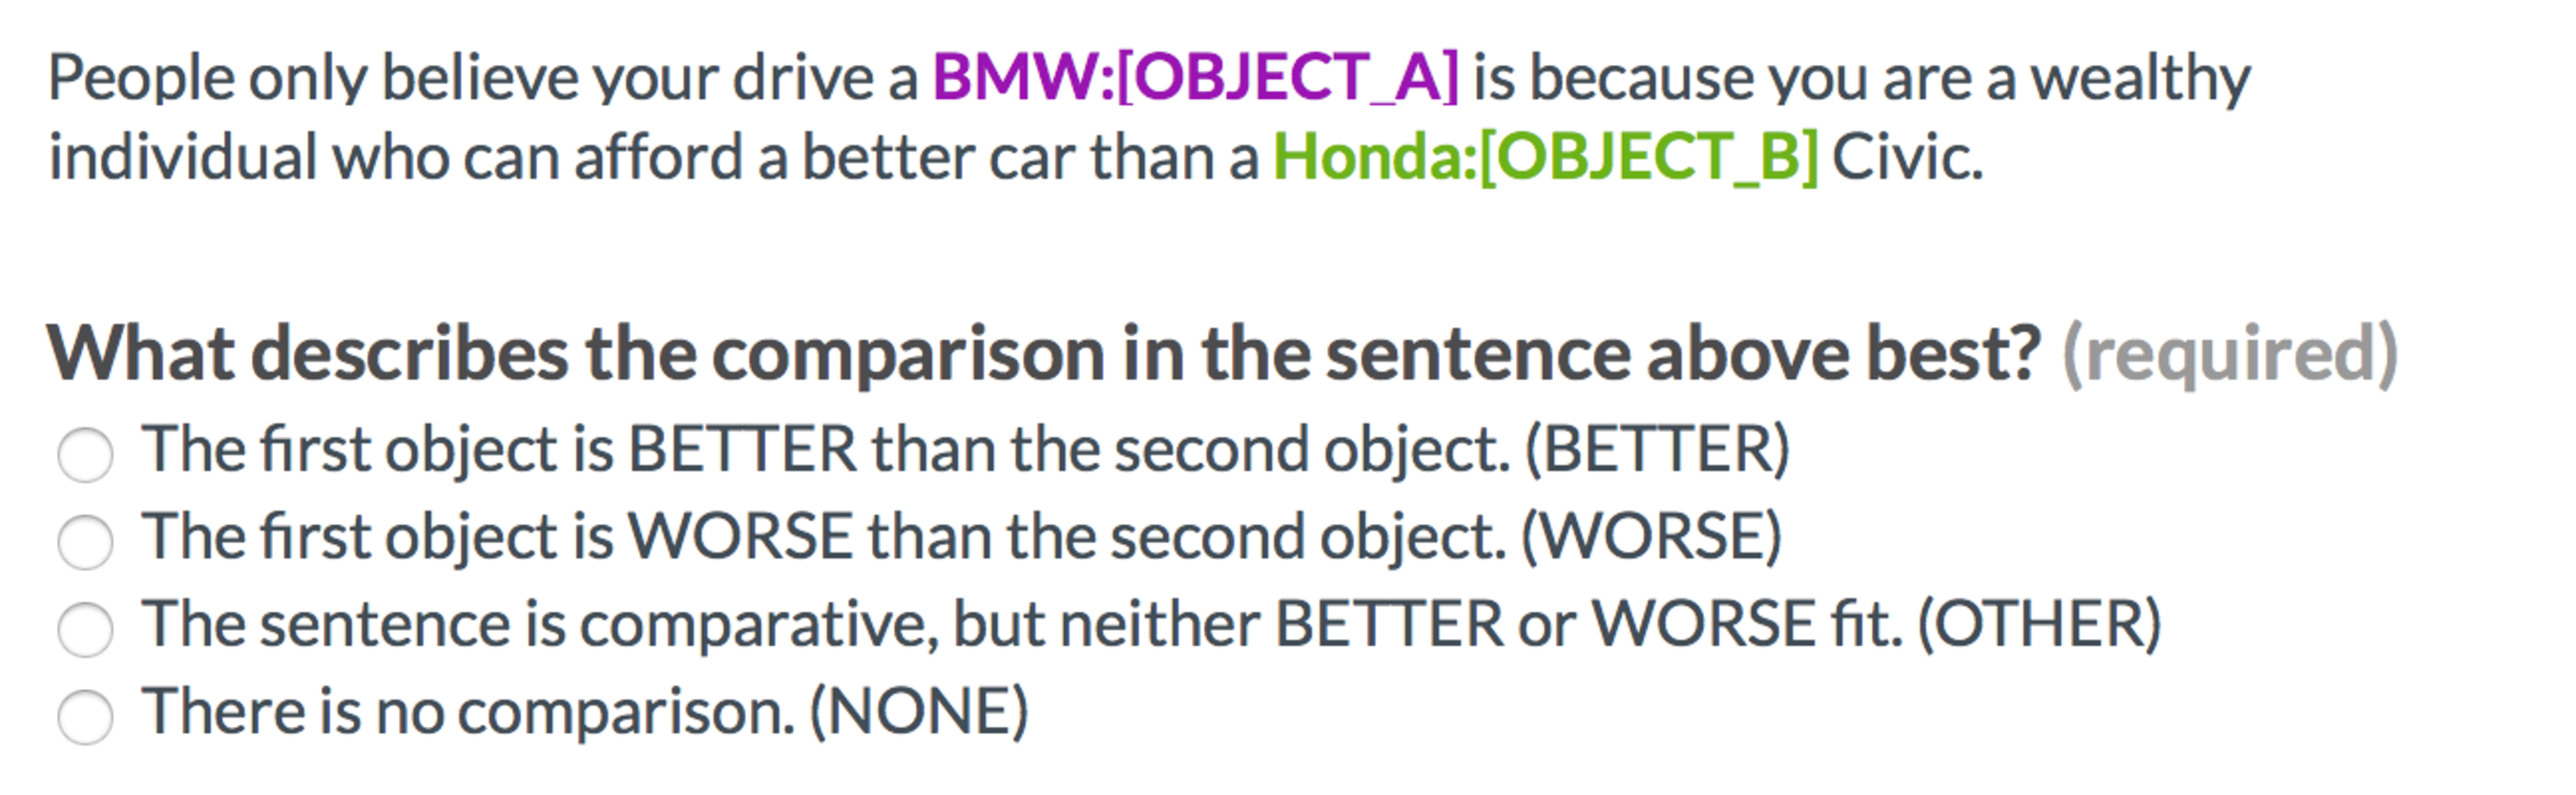
\includegraphics[scale=0.3]{images/q1other}
    \end{frame}


    \begin{frame}
        \frametitle{Task Design}
        \begin{itemize}
            \item After 750 annotated sentences per domain, \texttt{OTHER} was dropped
            \item People confused \texttt{OTHER} with \texttt{NONE} frequently
            \item People were dissatisfied because the distinction is to hard
            \item \texttt{OTHER} and \texttt{NONE} were hardly distinguishable in first classification experiments
            \item \texttt{OTHER} was merged into \texttt{NONE} for the classification experiments
        \end{itemize}
    \end{frame}


    \begin{frame}
        \frametitle{Results: Brands}
        \begin{center}
            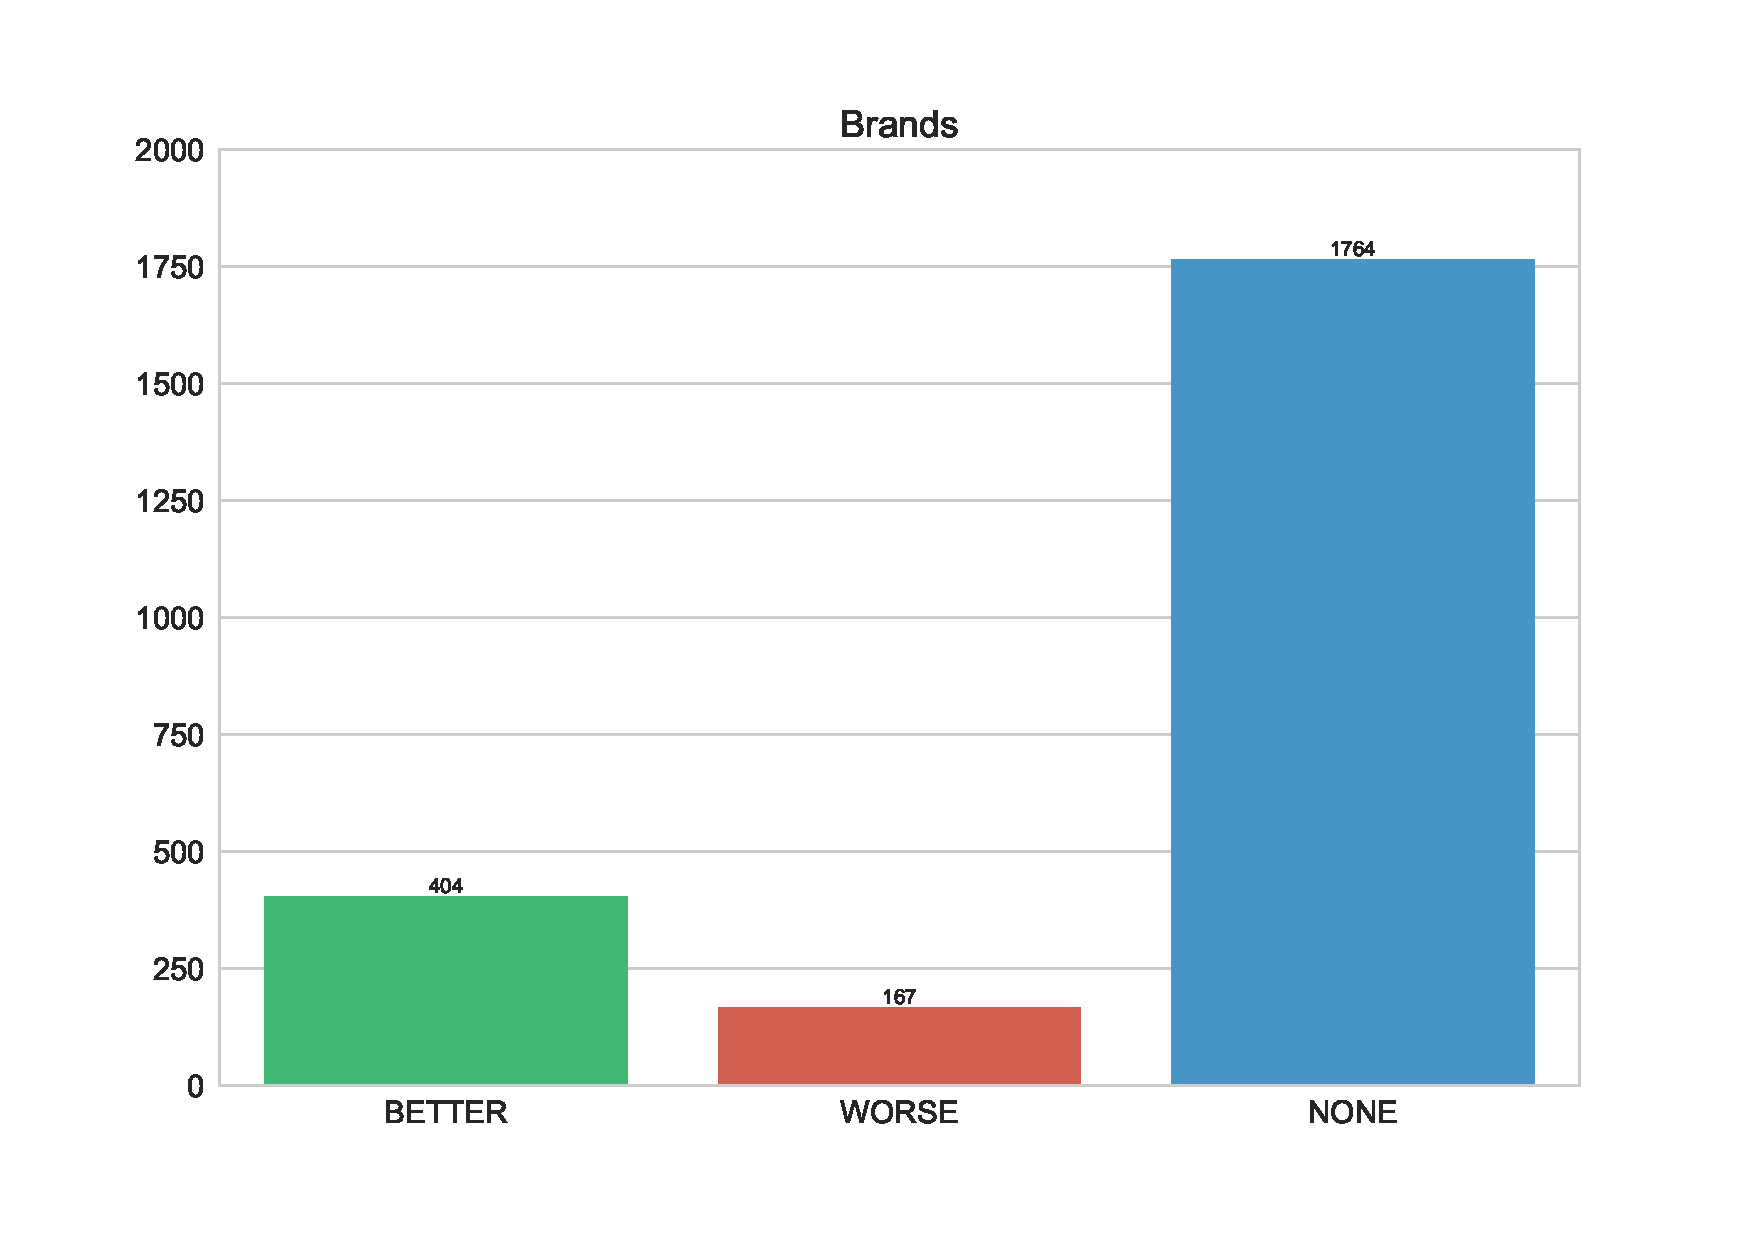
\includegraphics[scale=0.3]{images/Brands-dist}
        \end{center}
    \end{frame}

    \begin{frame}
        \frametitle{Results: Computer Science}
        \begin{center}
            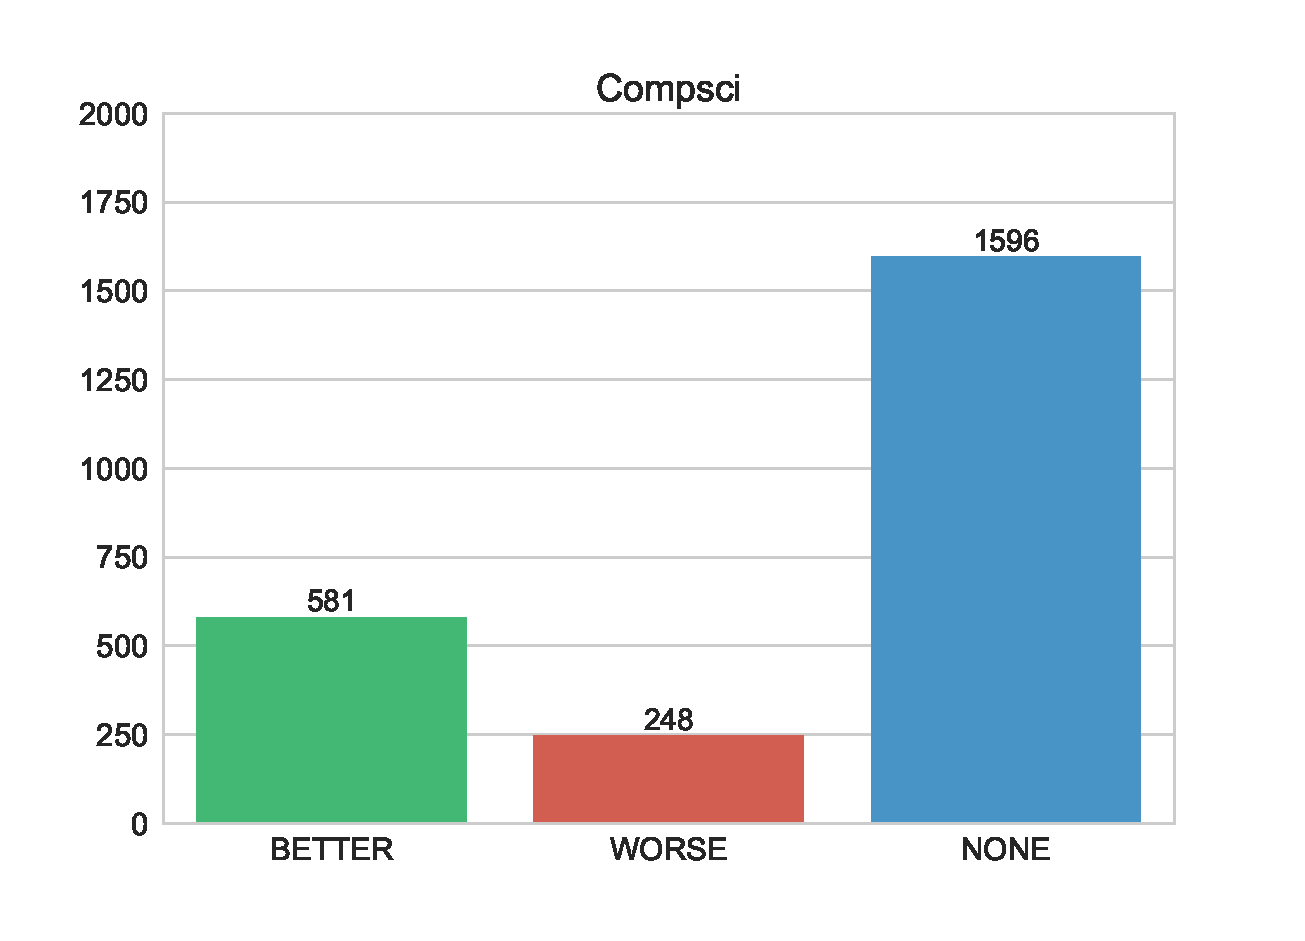
\includegraphics[scale=0.3]{images/Compsci-dist.pdf}
        \end{center}
    \end{frame}

    \begin{frame}
        \frametitle{Results: Random}
        \begin{center}
            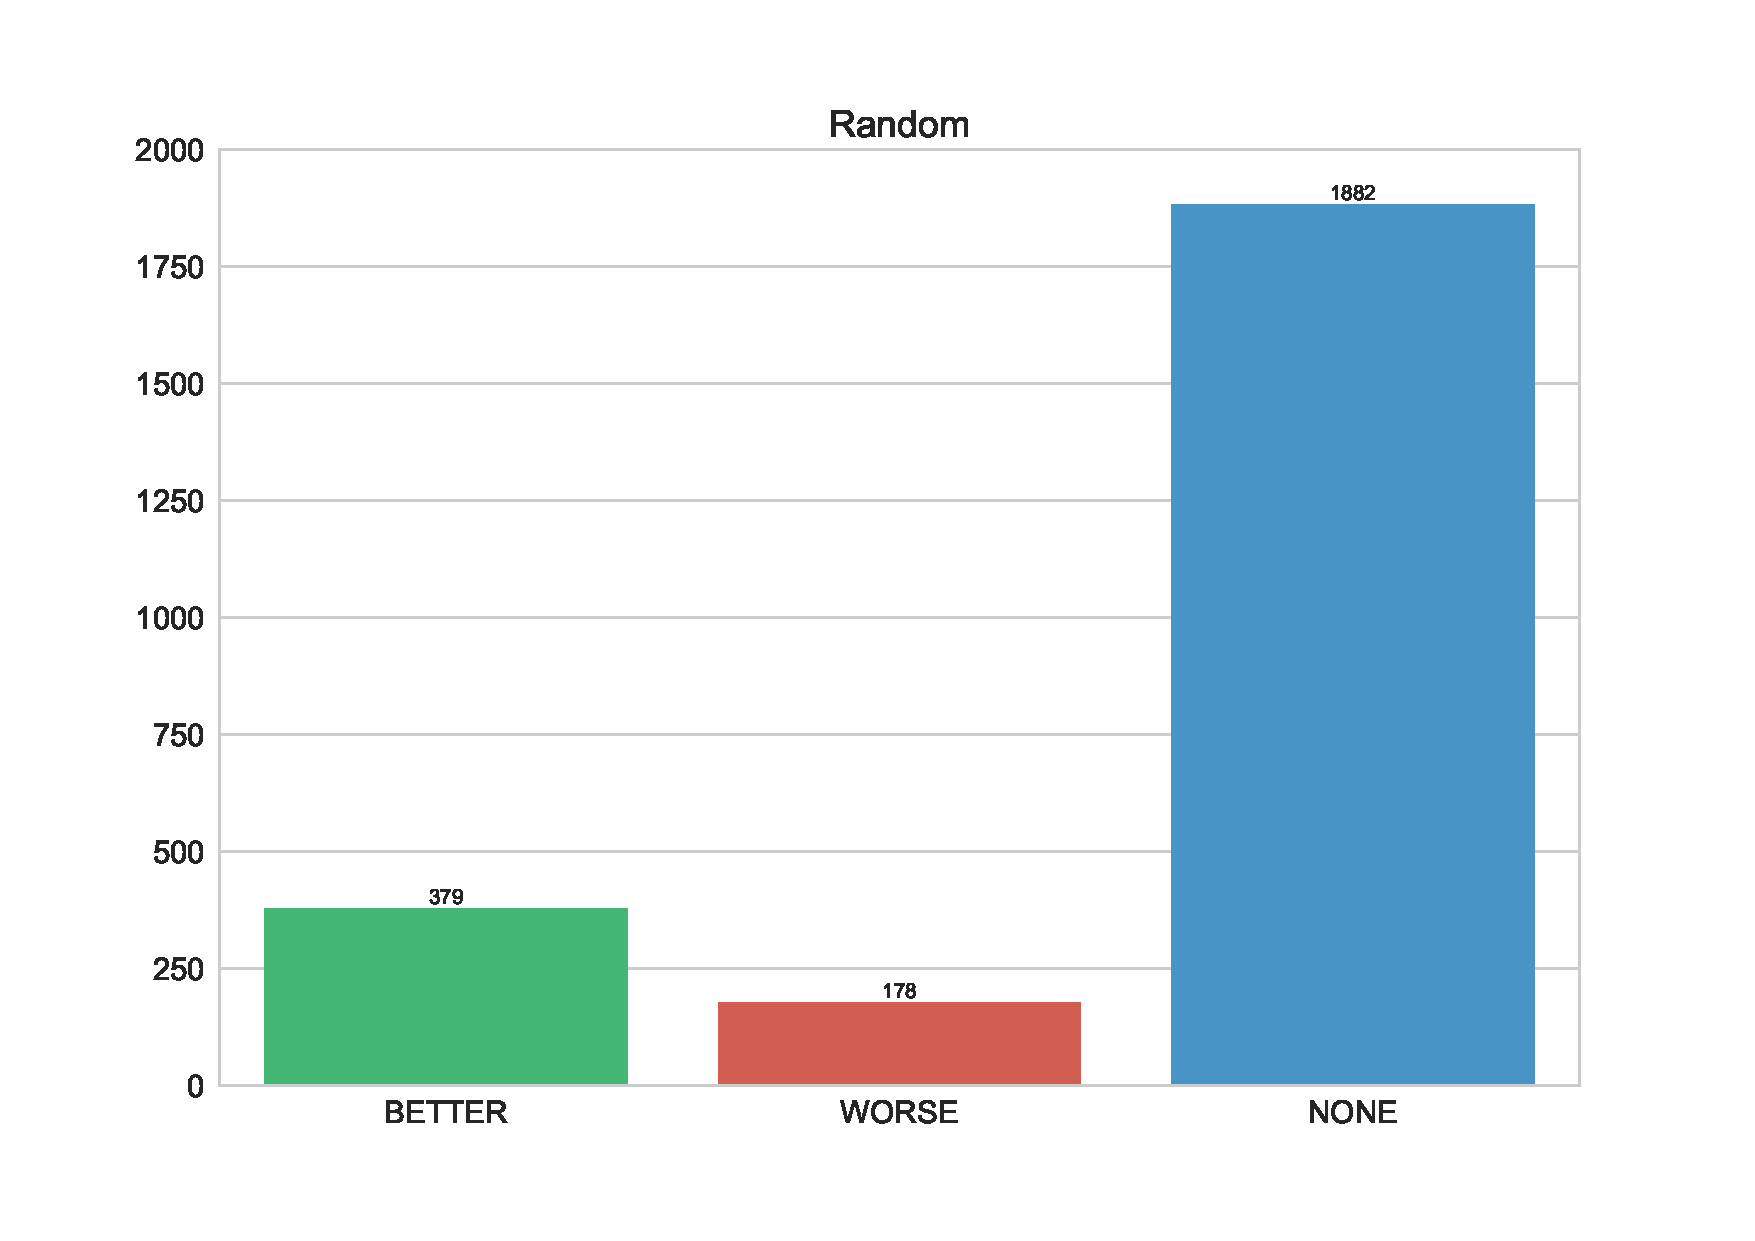
\includegraphics[scale=0.3]{images/Random-dist.pdf}
        \end{center}
    \end{frame}

    \begin{frame}
        \frametitle{Results: All}
        \begin{center}
            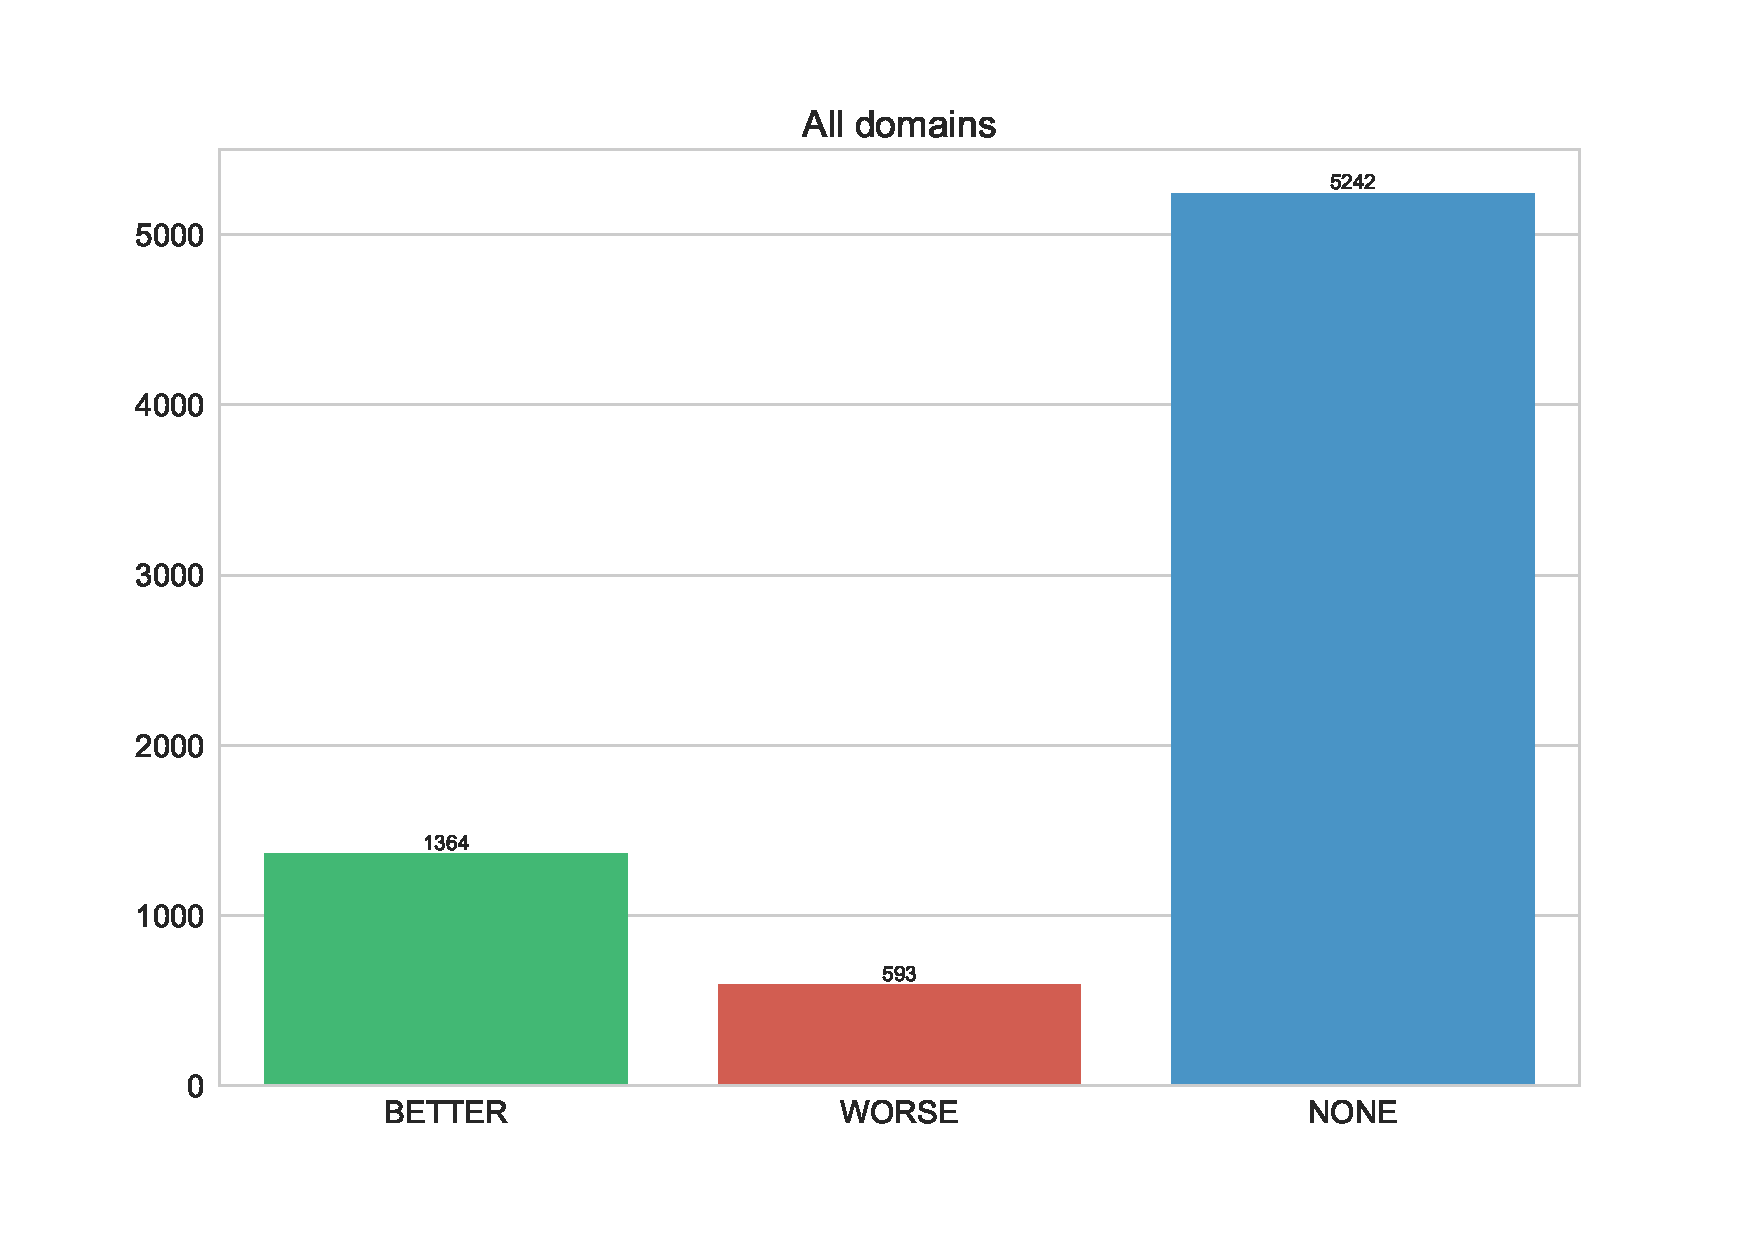
\includegraphics[scale=0.3]{images/Alldomains-dist.pdf}
        \end{center}
    \end{frame}

    \begin{frame}
        \frametitle{Results: Confidence}

        Annotation confidence for all domains. The confidence is calculated as $\nicefrac{\text{judgments for majority class}}{\text{total judgments}}$.

        \begin{center}
            \begin{tabular}{@{}rrr@{}}
                \toprule
                Confidence & Sentences & \% of data set \\
                \midrule
                100\%    & 5111 & 71.00     \\
                91-99\%    & 0 & 0.00     \\
                81-90\%    & 75 & 1.04     \\
                71-80\%    & 1057 & 14.68     \\
                61-70\%    & 33 & 0.46     \\
                51-60\%    & 754 & 10.47     \\
                0-50\%    & 169 & 2.35     \\
                \bottomrule
            \end{tabular}

        \end{center}
    \end{frame}

    \begin{frame}
        \frametitle{Results}
        \begin{itemize}
            \item 7199 annotated sentences
            \item 27 percent of the sentences are comparative
            \item The annotators agreed on the same class for 5111 sentences
            \item
        \end{itemize}
    \end{frame}

    \section{Classification}
    \frame{\sectionpage}
    \begin{frame}
        \frametitle{Algorithms}
        \begin{columns}[t]
            \column{2in}
            \begin{itemize}
                \item 13 classification algorithms were tested with a bag-of-words-model
                \item XGBoost (gradient boosted decision trees) worked best
                \item  The graphic shows the f1 score and standard derivation (black bar).
            \end{itemize}
            \column{3.5in}

            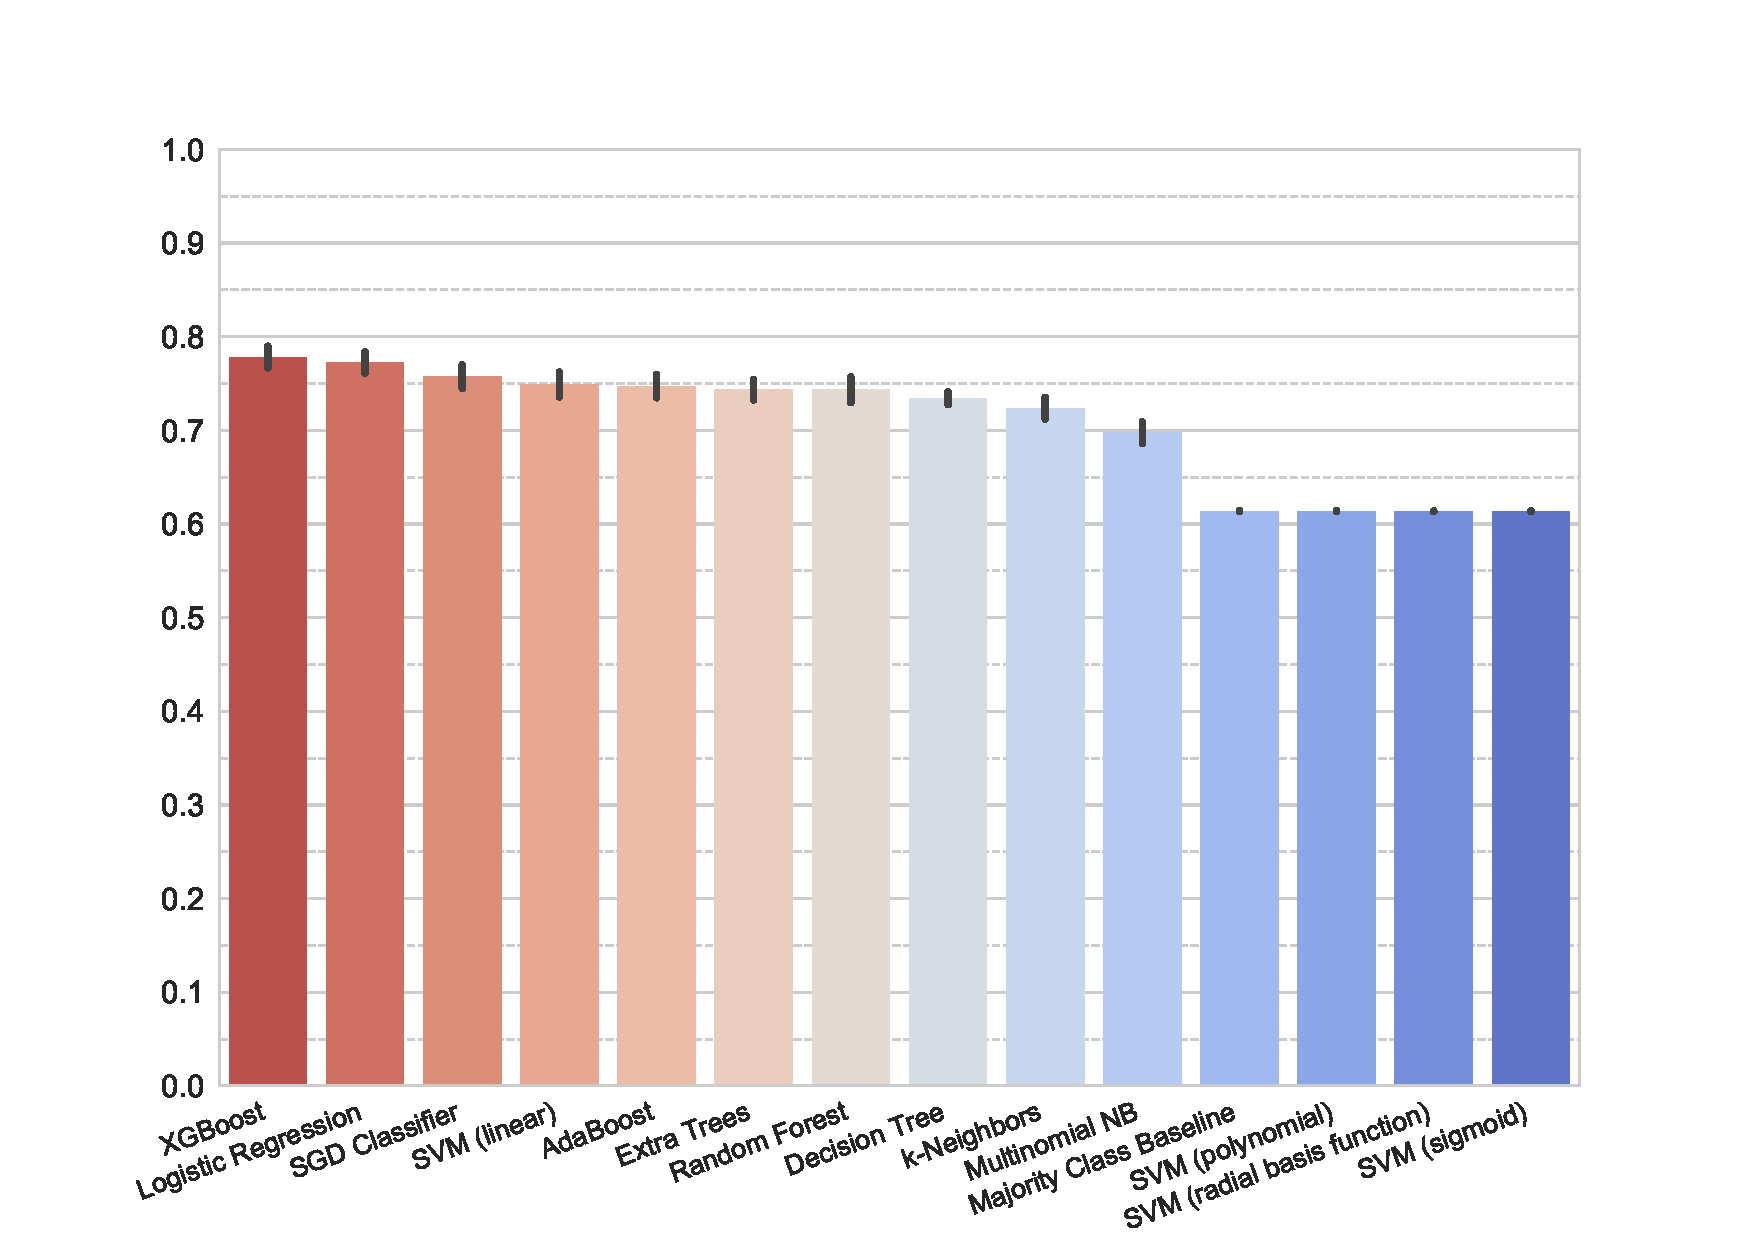
\includegraphics[scale=0.35,trim={1cm 0 0 5.45cm},clip]{images/classifier.pdf}


        \end{columns}
    \end{frame}

    \begin{frame}
        \frametitle{Setup}
        \begin{itemize}
            \item XGBoost with 1000 base estimators was used in all further experiments
            \item Exhaustive grid search and randomized search on XGBoost's parameters did not find better parameter values
            \item The 7199 sentences were split into a development (5759) and held-out (1440).
            \item All experiments were conducted on the development set and evalutated with k-folds cross validation ($k = 5$)
            \item Two setups: classification with three classes and binary classification (\texttt{BETTER} and \texttt{WORSE} were combined to \texttt{ARG})
        \end{itemize}

    \end{frame}

    \begin{frame}
        \frametitle{Baseline: Three classes}

        \begin{minipage}{.5\linewidth}
            \caption{Random (stratified) baseline}
            \label{tbl:3stratifiedbaseline}
            \centering

            \begin{tabularx}{0.97\linewidth}{Xrrrr}
                \toprule
                & precision & recall & f1 score                     \\ \midrule
                \texttt{B} & 0.19 \scriptsize{$\pm$0.01} & 0.21 \scriptsize{$\pm$0.01} & 0.20 \scriptsize{$\pm$0.01} \\
                \texttt{W}  & 0.06 \scriptsize{$\pm$0.02} & 0.05 \scriptsize{$\pm$0.02} & 0.06 \scriptsize{$\pm$0.03} \\
                \texttt{N}   & 0.73 \scriptsize{$\pm$0.00}  & 0.73 \scriptsize{$\pm$0.00} & 0.73 \scriptsize{$\pm$0.00} \\
                avg. & 0.57 \scriptsize{$\pm$0.00} & 0.58 \scriptsize{$\pm$0.01} & 0.57 \scriptsize{$\pm$0.00} \\
                \bottomrule
            \end{tabularx}

        \end{minipage}%
        \begin{minipage}{.5\linewidth}
            \centering
            \caption{Majority class baseline}
            \label{tbl:3majoritybaseline}
            \begin{tabularx}{0.97\linewidth}{Xrrrr}
                \toprule
                & precision & recall & f1 score                                    \\ \midrule
                \texttt{B} & 0.00 \scriptsize{$\pm$0.00} & 0.00 \scriptsize{$\pm$0.00} & 0.00 \scriptsize{$\pm$0.00}                \\
                \texttt{W}  & 0.00 \scriptsize{$\pm$0.00} & 0.00 \scriptsize{$\pm$0.00} & 0.00 \scriptsize{$\pm$0.00}                \\
                \texttt{N}   & 0.73 \scriptsize{$\pm$0.00}     & 1.00 \scriptsize{$\pm$0.00} & 0.84 \scriptsize{$\pm$0.00}                \\
                avg. & 0.53 \scriptsize{$\pm$0.00} & 0.73 \scriptsize{$\pm$0.00} & \textbf{0.61} \scriptsize{$\pm$0.00} \\
                \bottomrule
            \end{tabularx}
        \end{minipage}\newline\newline
        \texttt{B} = \texttt{BETTER}, \texttt{W} = \texttt{WORSE}, \texttt{N} = \texttt{NONE},
    \end{frame}

    \begin{frame}
        \frametitle{Baseline: Binary}


        \begin{minipage}{.5\linewidth}
            \caption{Random (stratified) baseline}
            \label{tbl:binmaj}
            \centering

            \begin{tabularx}{0.97\linewidth}{Xrrrr}
                \toprule
                & precision & recall & f1 score                              \\ \midrule
                \texttt{ARG}  & 0.26 \scriptsize{$\pm$0.03} & 0.26 \scriptsize{$\pm$0.03} & 0.26 \scriptsize{$\pm$0.03}          \\
                \texttt{N} & 0.72 \scriptsize{$\pm$0.01} & 0.72 \scriptsize{$\pm$0.01} & 0.72 \scriptsize{$\pm$0.01}          \\
                avg. & 0.60 \scriptsize{$\pm$0.02} & 0.60 \scriptsize{$\pm$0.02} & 0.60 \scriptsize{$\pm$0.02} \\
                \bottomrule
            \end{tabularx}

        \end{minipage}%
        \begin{minipage}{.5\linewidth}
            \centering
            \caption{Majority class baseline}
            \label{tbl:binstrat}
            \begin{tabularx}{0.97\linewidth}{Xrrrr}
                \toprule
                & precision & recall & f1 score                     \\ \midrule
                \texttt{ARG}  & 0.00 \scriptsize{$\pm$0.00} & 0.00 \scriptsize{$\pm$0.00} & 0.00 \scriptsize{$\pm$0.00} \\
                \texttt{N} & 0.73 \scriptsize{$\pm$0.00} & 1.00 \scriptsize{$\pm$0.00} & 0.84 \scriptsize{$\pm$0.00} \\
                avg. & 0.53 \scriptsize{$\pm$0.00} & 0.73 \scriptsize{$\pm$0.00} & \textbf{0.61} \scriptsize{$\pm$0.00} \\
                \bottomrule
            \end{tabularx}
        \end{minipage}\newline\newline
        \texttt{ARG} = \texttt{BETTER} + \texttt{WORSE}, \texttt{N} = \texttt{NONE}


    \end{frame}

    \subsection{Features}
    %    \begin{frame}
    %        \frametitle{Sentence Embeddings}
    %
    %    \end{frame}
    %
    %    \begin{frame}
    %        \frametitle{LexNet: Dependency Path I}
    %
    %    \end{frame}

    \begin{frame}
        \frametitle{Other features}
        \begin{itemize}
            \item Bag-of-words
            \item 500 most frequent part-of-speech bi-, tri and four-grams
            \item Mean word embedding vector (GloVe embeddings)
            \item Boolean feature capturing the appearance of a comparative adjective
        \end{itemize}

    \end{frame}

    \subsection{Training Results}
    \begin{frame}
        \frametitle{Three classes: F1 score}
        \centerline{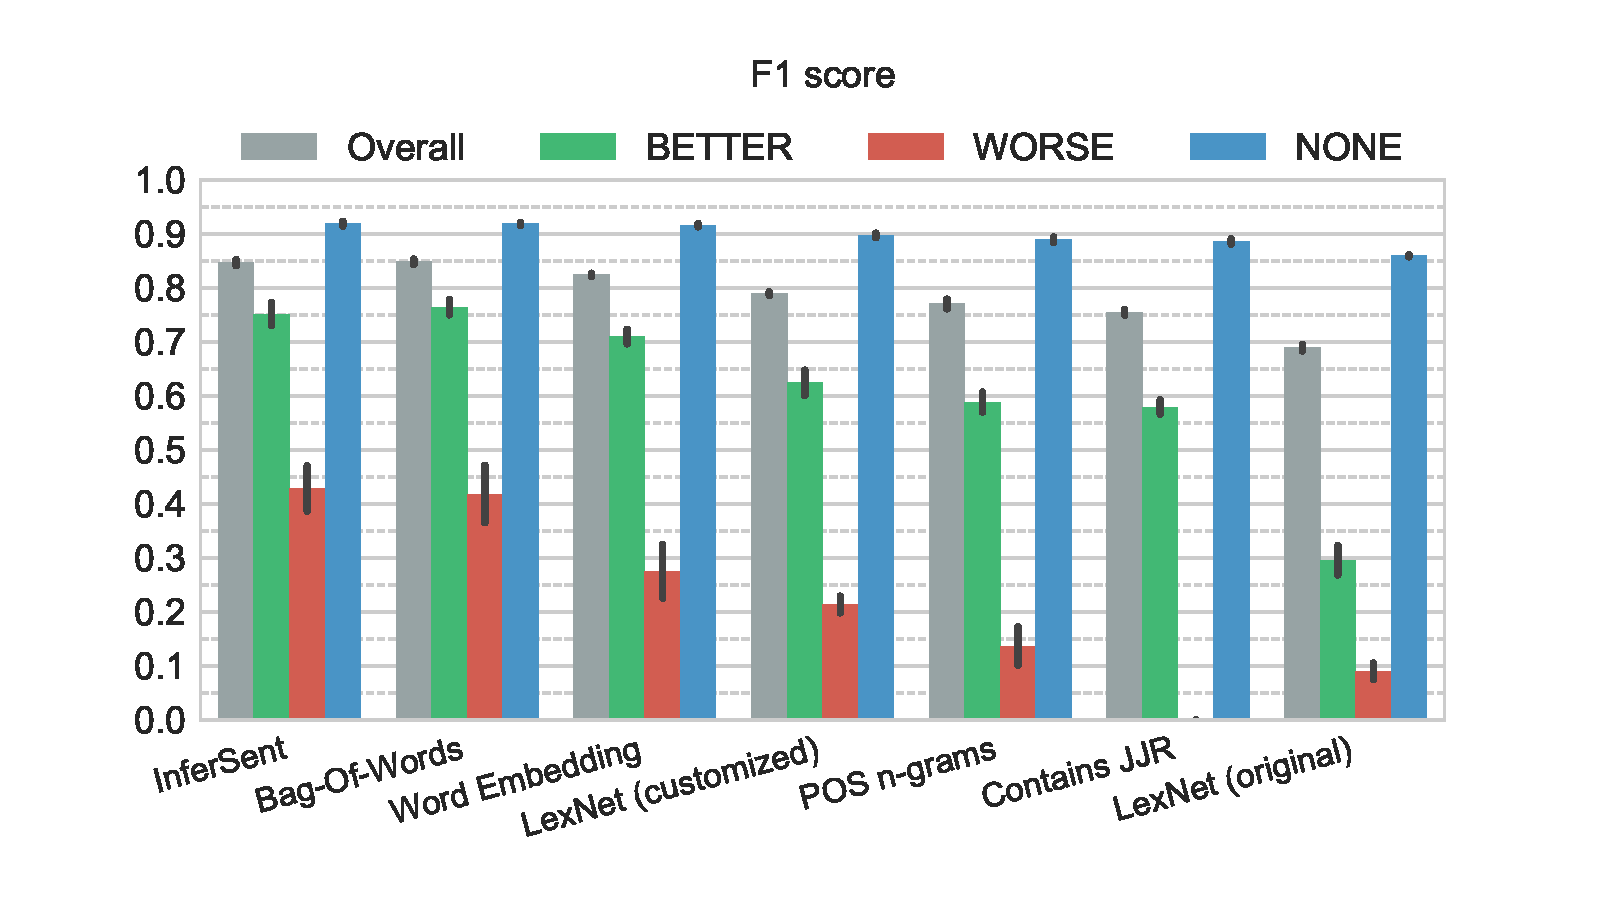
\includegraphics[scale=0.45,trim={0 0 0 0.5cm},clip]{images/experiments/p-f1-False}}
    \end{frame}


    \begin{frame}
        \frametitle{Three classes: Precision and Recall}
        \begin{columns}[t]
            \column{2in}
            \centerline{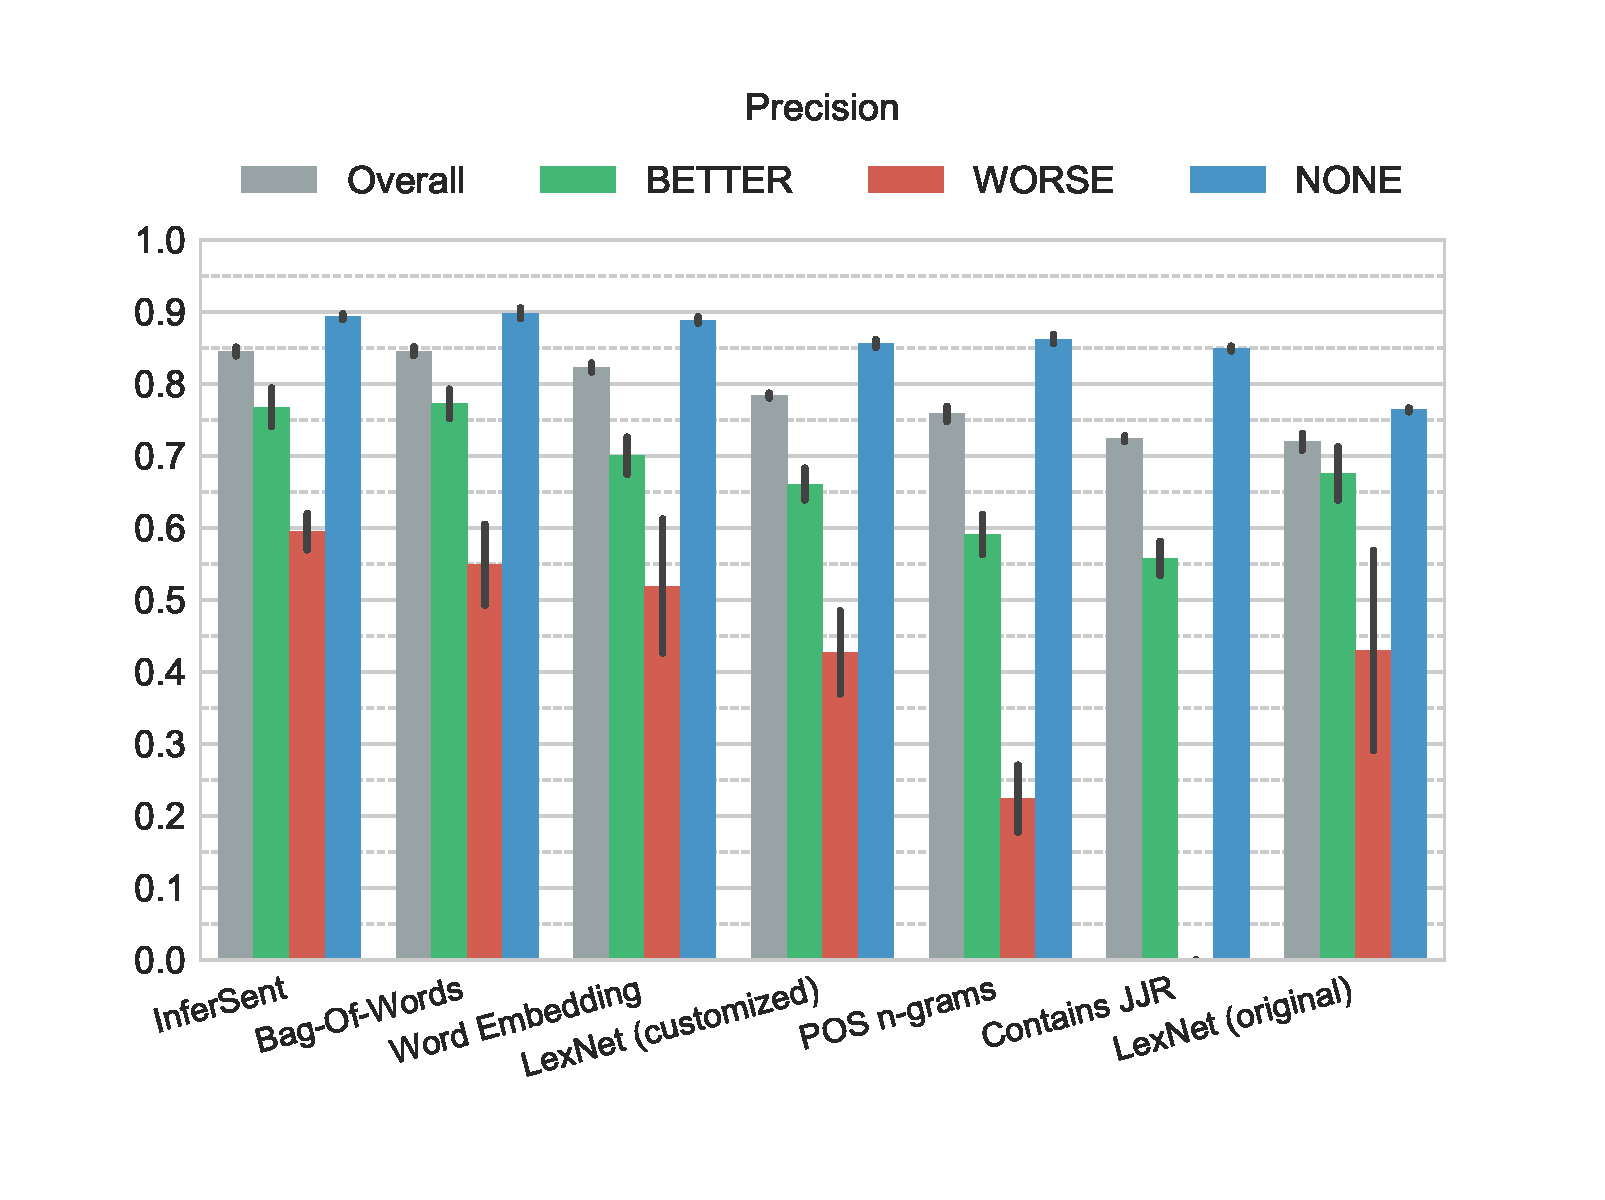
\includegraphics[scale=0.31,trim={2cm 0 0 0},clip]{images/experiments/p-precision-False}}
            \column{2in}
            \centerline{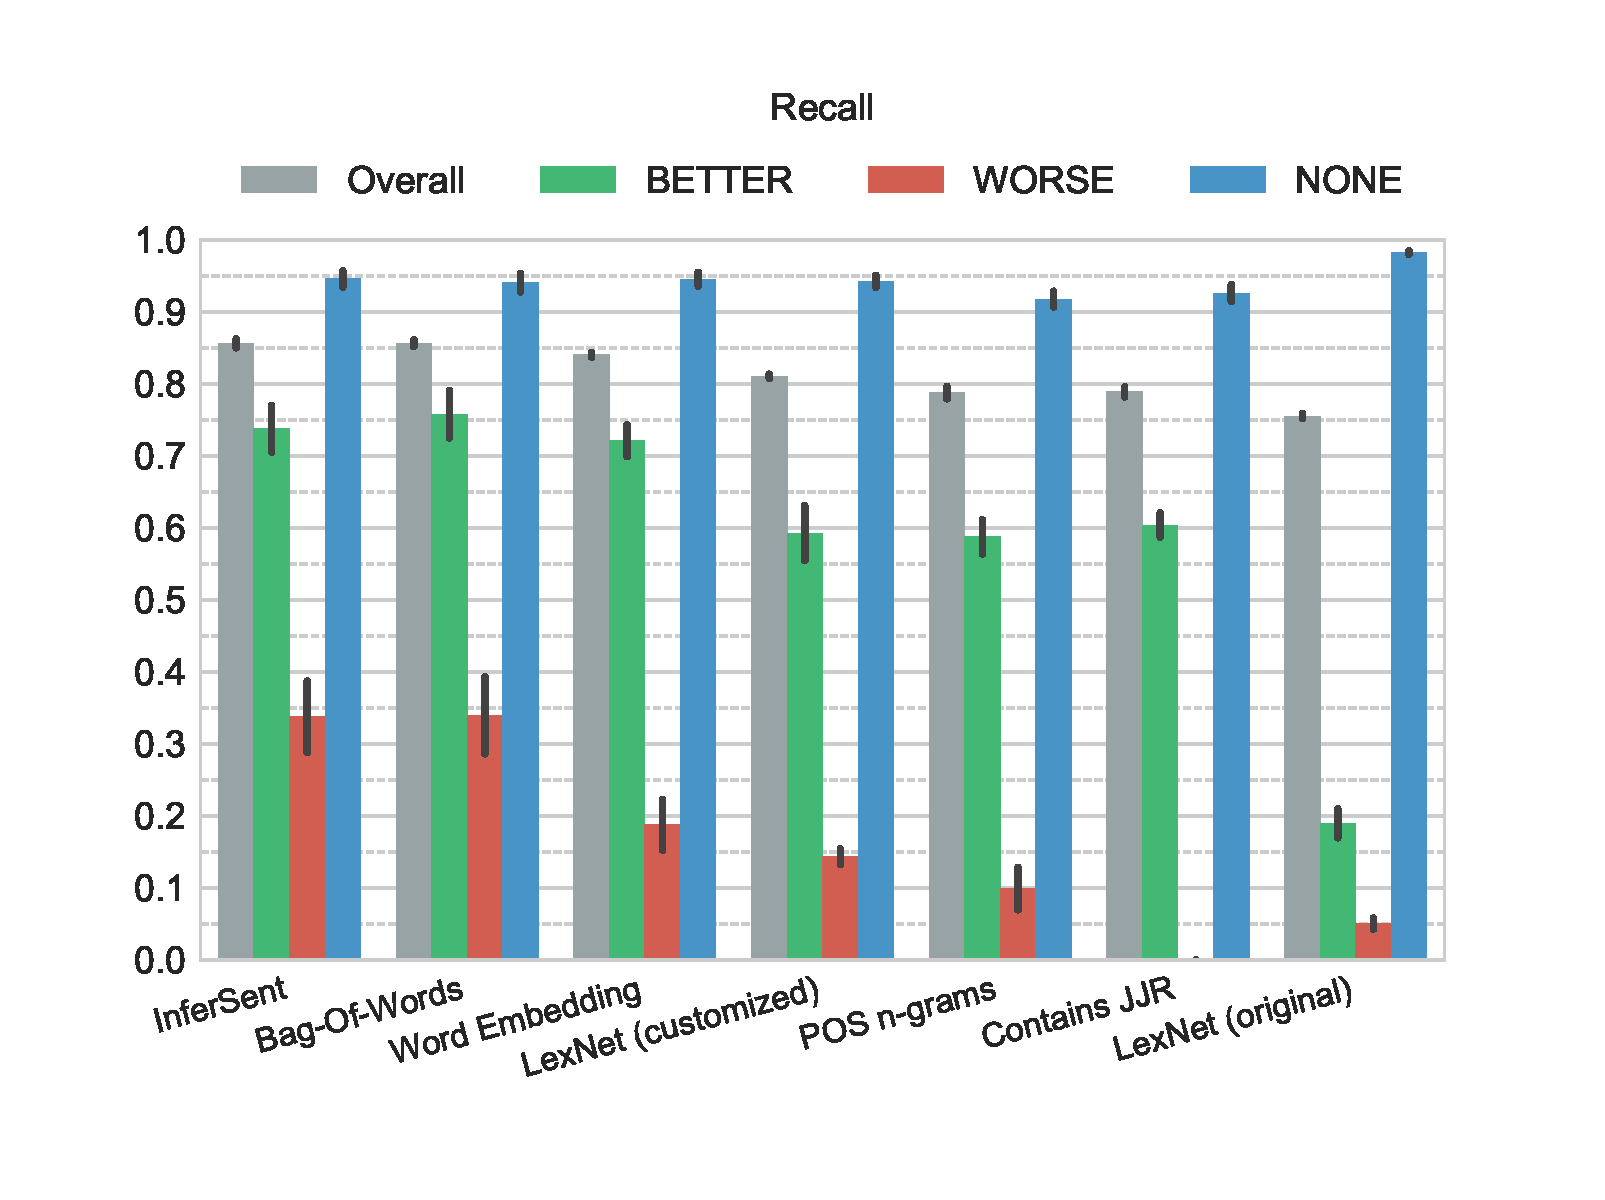
\includegraphics[scale=0.31,trim={0 0 2cm 0},clip]{images/experiments/p-recall-False}}

        \end{columns}
    \end{frame}

    \begin{frame}
        \frametitle{Binary: F1 score}
        \centerline{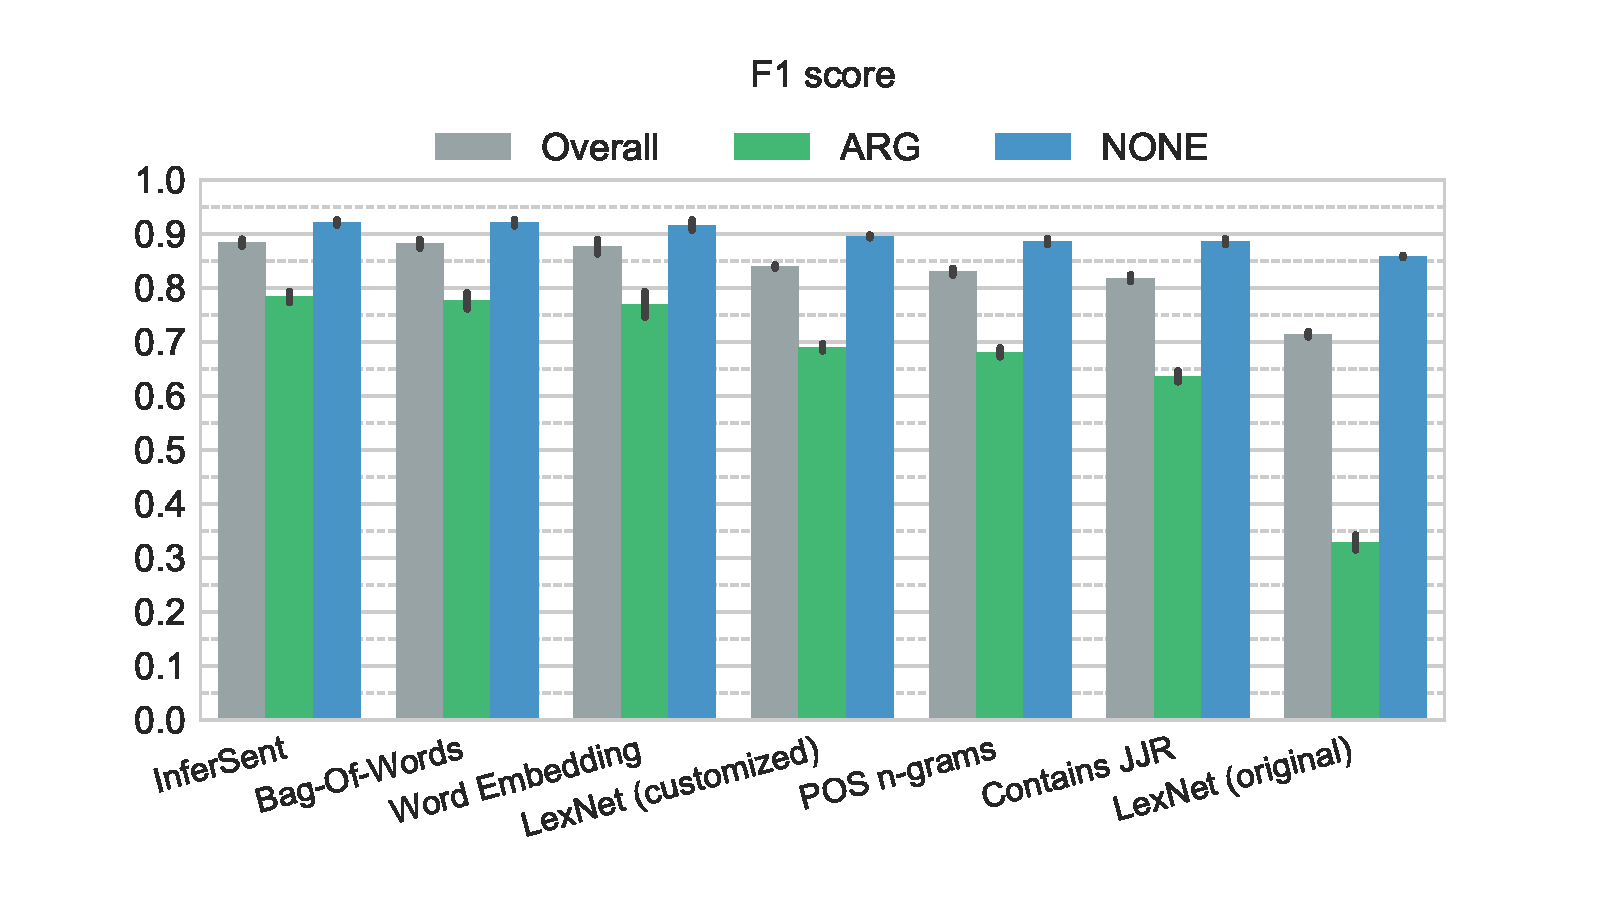
\includegraphics[scale=0.45,trim={0 0 0 0.5cm},clip]{images/experiments/p-f1-True}}
    \end{frame}


    \begin{frame}
        \frametitle{Binary: Precision and Recall}
        \begin{columns}[t]
            \column{2in}
            \centerline{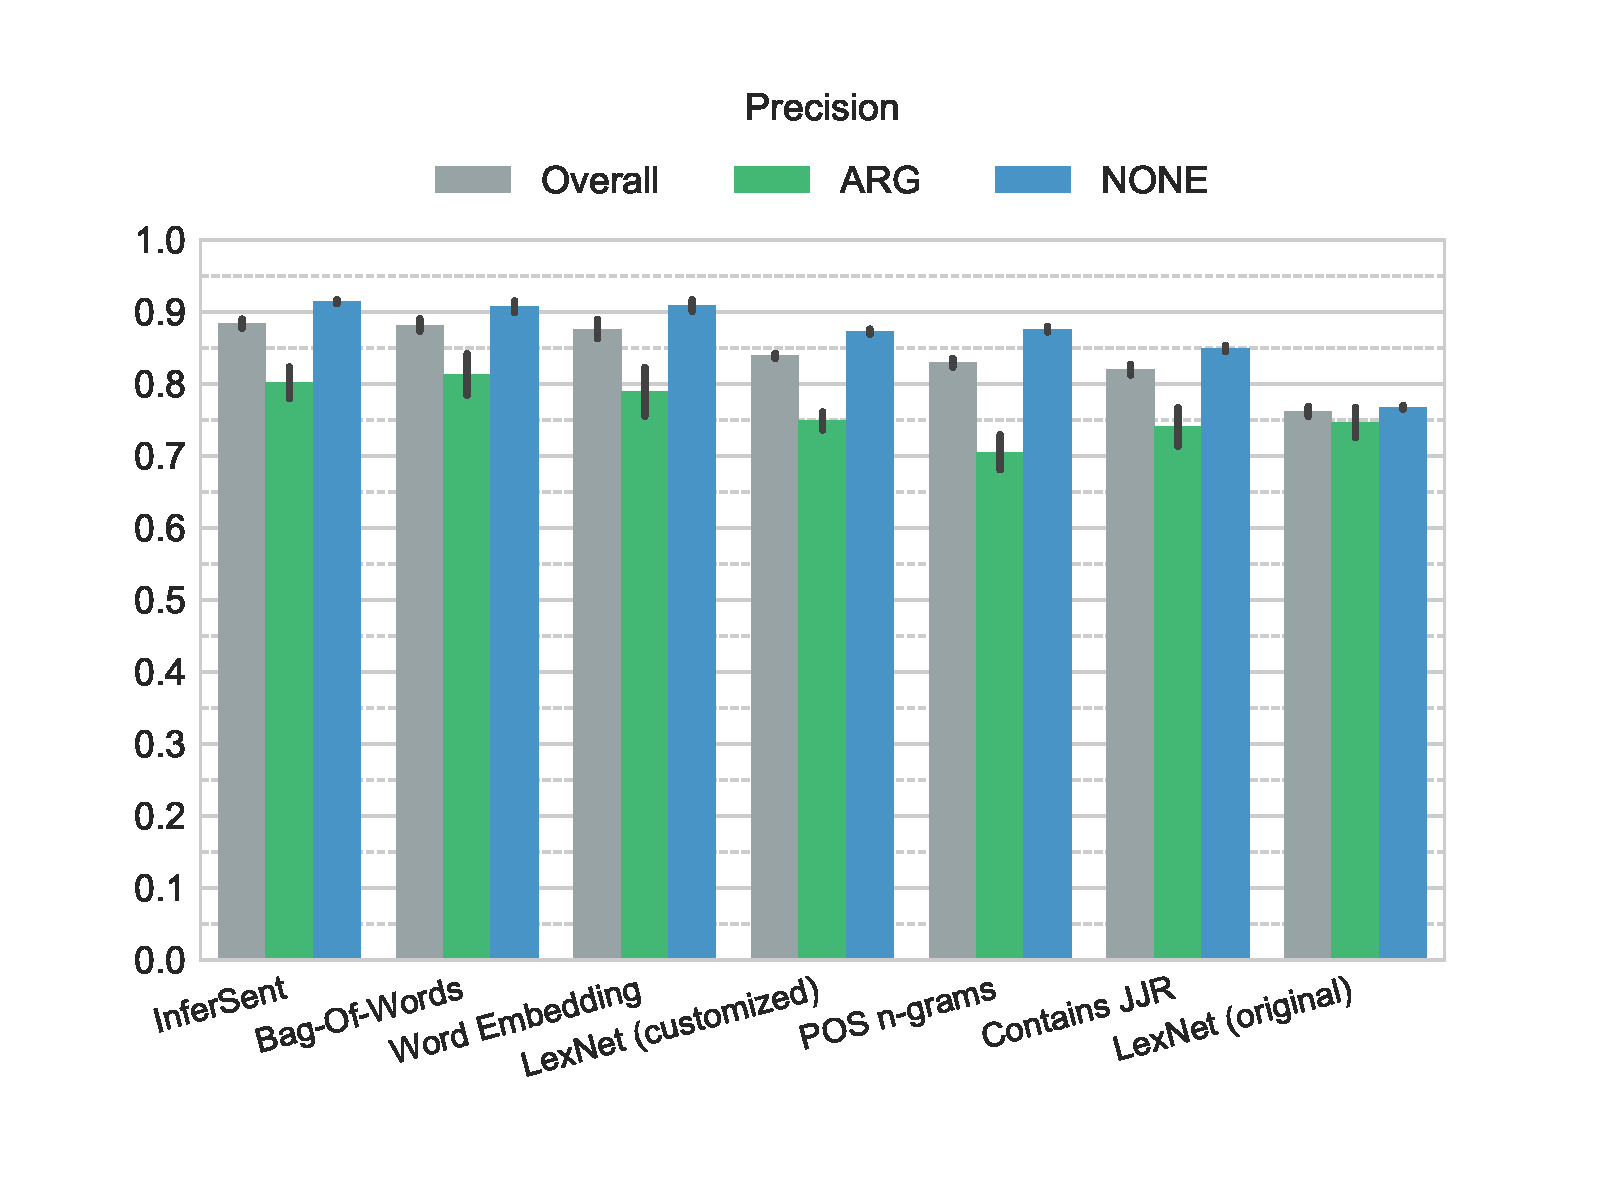
\includegraphics[scale=0.31,trim={2cm 0 0 0},clip]{images/experiments/p-precision-True}}
            \column{2in}
            \centerline{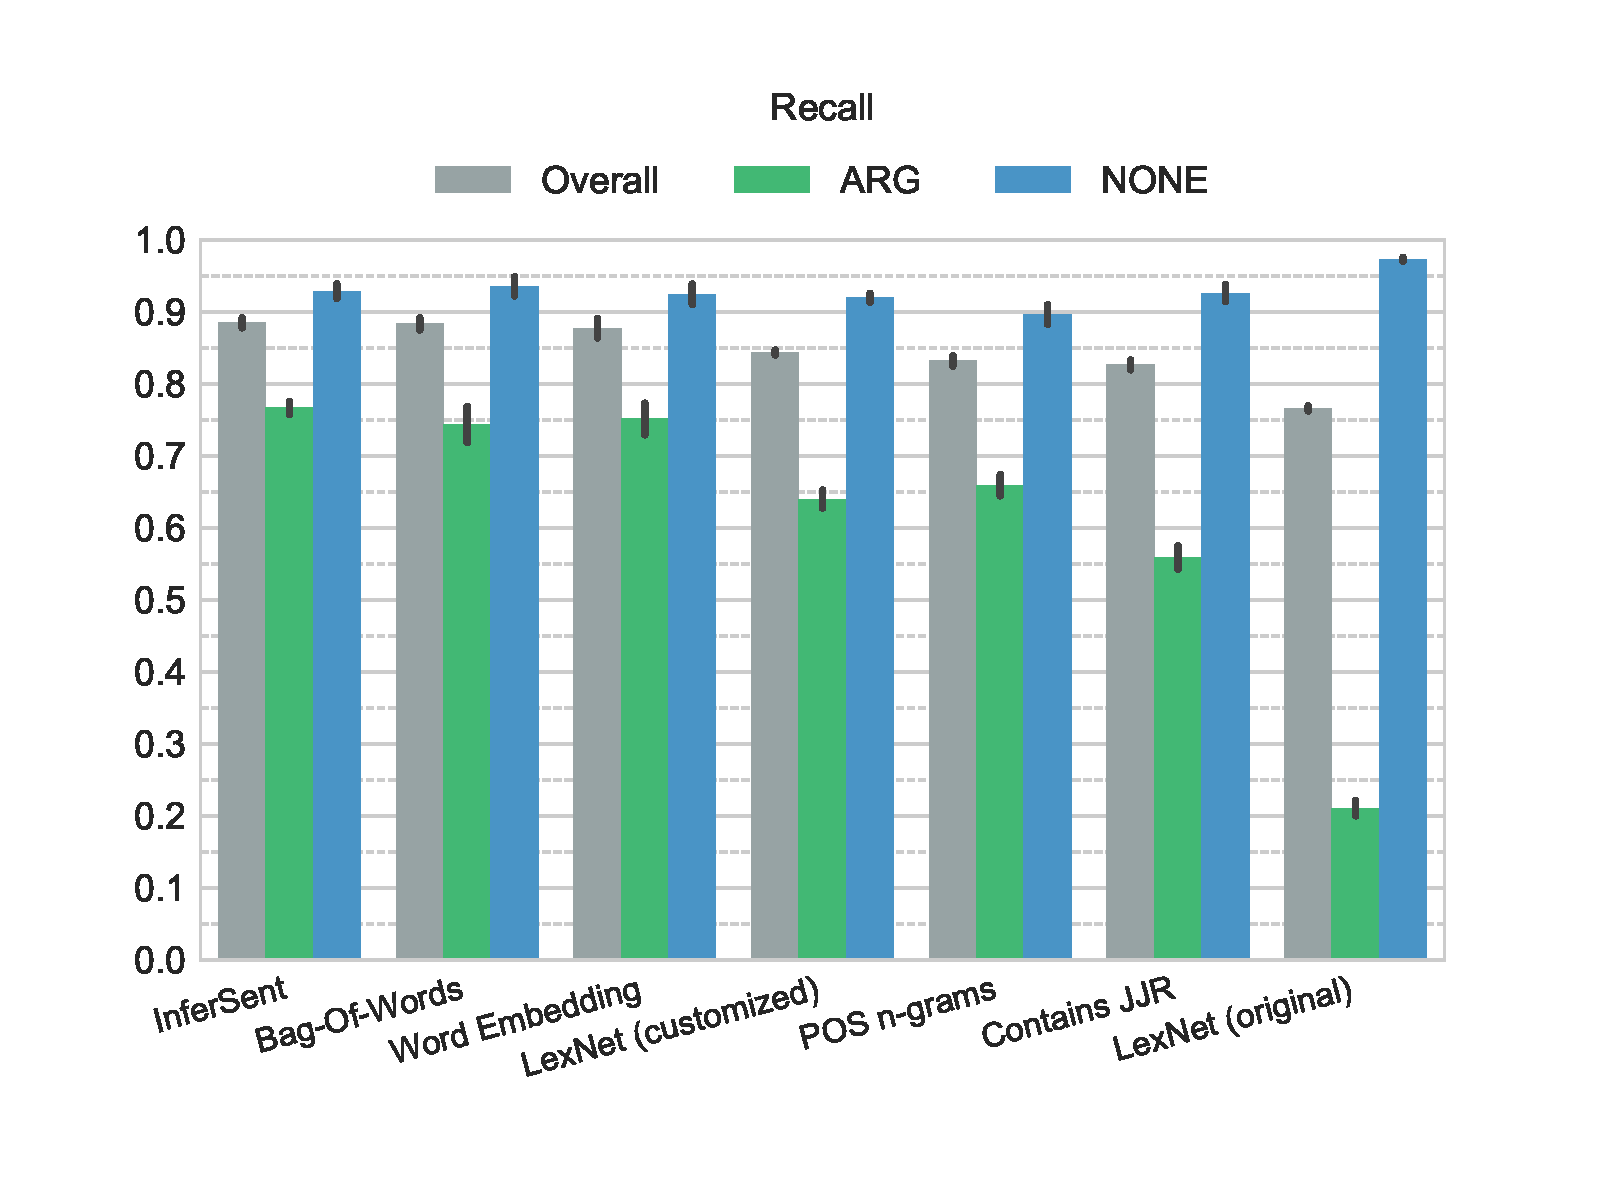
\includegraphics[scale=0.31,trim={0 0 2cm 0},clip]{images/experiments/p-recall-True}}

        \end{columns}
    \end{frame}



    \section{Discussion and Future Work}
    \frame{\sectionpage}
    \begin{frame}
        \frametitle{abc}

    \end{frame}

\end{document}